\subsection{Data Collection}
The data taken was for the variables in equation \ref{eq:NozzleForce}. There were a total of 10 nozzle expansion ratios used with 2 trials each. The expansion ratio kept $A_t$ constant and varied $A_e$. There were 4 over expanded, 4 underexpanded, 1 optimum, and 1 with no expansion. The naming scheme goes something like ERT, where E stands for either U (Underexpanded), N (None), or O. O stands for either optimum or overexpanded. R is the ratio number (1-4) except in the case that there is no third character. In this case the O stands for optimum, which there is only one of. T stands for trial number which can be either 1 or 2. So for example, U22 is underexpanded, ratio number 2, trial number 2. O1 is optimum ratio, trial number 1. These are explicitly defined in the nomenclature section \ref{nomenclature}.%
\nomenclature{$O11$}{Overexpanded area ratio 1, trial 1}%
\nomenclature{$O12$}{Overexpanded area ratio 1, trial 2}%
\nomenclature{$O21$}{Overexpanded area ratio 2, trial 1}%
\nomenclature{$O22$}{Overexpanded area ratio 2, trial 2}%
\nomenclature{$O31$}{Overexpanded area ratio 3, trial 1}%
\nomenclature{$O32$}{Overexpanded area ratio 3, trial 2}%
\nomenclature{$O41$}{Overexpanded area ratio 4, trial 1}%
\nomenclature{$O42$}{Overexpanded area ratio 4, trial 2}%
\nomenclature{$U11$}{Underexpanded area ratio 1, trial 1}%
\nomenclature{$U12$}{Underexpanded area ratio 1, trial 2}%
\nomenclature{$U21$}{Underexpanded area ratio 2, trial 1}%
\nomenclature{$U22$}{Underexpanded area ratio 2, trial 2}%
\nomenclature{$U31$}{Underexpanded area ratio 3, trial 1}%
\nomenclature{$U32$}{Underexpanded area ratio 3, trial 2}%
\nomenclature{$U41$}{Underexpanded area ratio 4, trial 1}%
\nomenclature{$U42$}{Underexpanded area ratio 4, trial 2}%
\nomenclature{$O1$}{Optimum area ratio, trial 1}%
\nomenclature{$O2$}{Optimum area ratio, trial 2}%
\nomenclature{$N1$}{No expansion, trial 1}%
\nomenclature{$N2$}{No expansion, trial 2}
This naming scheme will be upated in future experiments because it was slightly problematic in the analysis of the data.
\begin{tcolorbox}[breakable,title=Data Sensors, height fixed for=first and middle]
There should be some light discussion on the sensors used for data collection. There was a single pressure transducer located near the inlet of the nozzle, a thermocouple located on the nozzle, a thermocouple located inside of the adaptor that the $CO_2$ connected to the rest of the plumbing, and a load cell setup to measure the thrust produced from the CGT. For sake of simplicity I will refer to these as "sensors" preceeded by the variable they measured. So, respectively, $P_c$ sensor, $T_e$ sensor, $T_c$ sensor, and $F$ sensor. Additionally, $\gamma$ is dependent on temperature, but only changes slighty in the temperature differences noticed here. In later models, $\gamma$ will be set to be a function of temperature for greater accuracy. For now it is not necessary because the force has a small dependence on $\gamma$ compared to the temperature . So, for the sake of this project $\gamma$ is a constant. The data acquisition system was running python on a RaspberryPi 3 and since all of these sensors are analog devices 2 different analog-to-digital converters (ADCs) was used to interface with the Pi. The $P_c$, $T_e$, and $T_c$ sensors interfaced with a 10-bit ADC and the $F$ sensor interfaced with a 24-bit ADC. In future experiments, a 24-bit ADC will be used for all data acquisition because of the limited resolution with the 10-bit ADC. This is especially evident with the thermocouple data. All of the python scripts for data collection are available at my \href{https://github.com/maxmhuggins/RCS_HAB/tree/master/On_Ground_Testing/Code}{GitHub repository}.
\end{tcolorbox}
The code began the experiment after all sensors were calibrated and functioning properly. Data collection ran until the force production was below a certain threshold for a predefined number of points. This would also need to be updated because often times the force sensor would lose its zero position so defining the threshold value was not so easy. A better method would be using the change in force to determine when the experiment was over. This would work well because the force is transient until the $CO_2$ was all spent. After it was over the mass of the $CO_2$ canister was measured. All of this data was written to two seperate .txt files. One included the calibration values for the sensors and changes in mass, the other included $P_c$, $T_c$, $T_e$, and $F$. The previous was not recorded in a useful format and later work had to be done to resolve this. In the future this should be updated. The latter was simply comma delimited and worked fine for reading into python for analysis. The data files can be found at my \href{https://github.com/maxmhuggins/RCS_HAB/tree/master/On_Ground_Testing/Data_and_Analysis/Experimental_Data_Analysis/Refined_Data_Files}{GitHub repository} as well.
\subsection{Data Analysis}
To begin the analysis, simple plots were made to look at the sensor data over time. Immediately, it was found that the temperature data is quite poor! The resolution of the ADC is evident in the discrete steps that the temperature takes. Figure \ref{fig:BadTemp} shows an example of the temperature data.
\begin{figure}[h!]
\centering
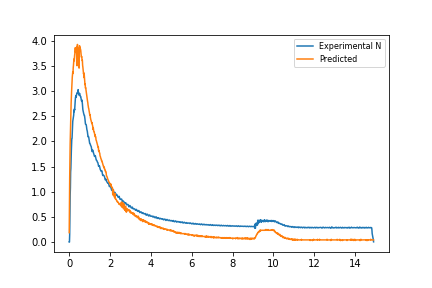
\includegraphics[scale=.5]{Figures/ExampleTemp}
\caption{Example plot of the temperature over time for a trial}
\label{fig:BadTemp}
\end{figure}